\documentclass[12pt, openany]{book}

% ──────────────────────────────────────────────
% Packages
% ──────────────────────────────────────────────
\usepackage[margin=1in]{geometry}
\usepackage{amsmath, amssymb, amsthm}
\usepackage{mathtools}
\usepackage{bm}
\usepackage{graphicx}
\usepackage{tikz}
\usepackage{pgfplots}
\pgfplotsset{compat=1.18}
\usetikzlibrary{arrows.meta, decorations.markings, calc, patterns, positioning}
\usepackage{tcolorbox}
\tcbuselibrary{theorems, breakable, skins}
\usepackage{hyperref}
\usepackage{enumitem}
\usepackage{fancyhdr}
\usepackage{titlesec}
\usepackage{epigraph}
\usepackage{xcolor}

% ──────────────────────────────────────────────
% Colors
% ──────────────────────────────────────────────
\definecolor{chapblue}{RGB}{0, 70, 130}
\definecolor{accentred}{RGB}{180, 40, 40}
\definecolor{softgray}{RGB}{245, 245, 245}
\definecolor{trajgreen}{RGB}{30, 130, 60}
\definecolor{darkgold}{RGB}{160, 120, 20}

% ──────────────────────────────────────────────
% Theorem environments
% ──────────────────────────────────────────────
\newtcbtheorem[number within=chapter]{principle}{Principle}{
  colback=chapblue!5, colframe=chapblue!80,
  fonttitle=\bfseries, separator sign={.~},
  breakable
}{princ}

\newtcbtheorem[number within=chapter]{keyidea}{Key Idea}{
  colback=accentred!5, colframe=accentred!70,
  fonttitle=\bfseries, separator sign={.~},
  breakable
}{idea}

\newtcbtheorem[number within=chapter]{example}{Example}{
  colback=softgray, colframe=black!40,
  fonttitle=\bfseries, separator sign={.~},
  breakable
}{ex}

\newtcbtheorem[number within=chapter]{definition}{Definition}{
  colback=darkgold!5, colframe=darkgold!80,
  fonttitle=\bfseries, separator sign={.~},
  breakable
}{def}

\theoremstyle{plain}
\newtheorem{proposition}{Proposition}[chapter]

% ──────────────────────────────────────────────
% Chapter formatting
% ──────────────────────────────────────────────
\titleformat{\chapter}[display]
  {\normalfont\huge\bfseries\color{chapblue}}
  {\chaptertitlename\ \thechapter}{20pt}{\Huge}
\titlespacing*{\chapter}{0pt}{-20pt}{30pt}

% ──────────────────────────────────────────────
% Header/Footer
% ──────────────────────────────────────────────
\pagestyle{fancy}
\fancyhf{}
\fancyhead[LE,RO]{\thepage}
\fancyhead[RE]{\textit{Control Is Motion}}
\fancyhead[LO]{\textit{\nouppercase{\leftmark}}}
\renewcommand{\headrulewidth}{0.4pt}
\setlength{\headheight}{14.5pt}

% ──────────────────────────────────────────────
% Custom commands
% ──────────────────────────────────────────────
\newcommand{\state}{\bm{x}}
\newcommand{\control}{\bm{u}}
\newcommand{\traj}{\bm{\gamma}}
\newcommand{\manifold}{\mathcal{M}}
\newcommand{\configspace}{\mathcal{Q}}
\newcommand{\statespace}{\mathcal{X}}
\newcommand{\controlspace}{\mathcal{U}}
\newcommand{\tube}{\mathcal{T}}
\newcommand{\Reals}{\mathbb{R}}
\newcommand{\dd}{\mathrm{d}}
\newcommand{\dt}{\,\dd t}
\newcommand{\norm}[1]{\left\lVert #1 \right\rVert}

% ──────────────────────────────────────────────
\title{%
  \vspace{-1cm}
  {\color{chapblue}\rule{\textwidth}{2pt}}\\[0.8cm]
  {\Huge\bfseries\color{chapblue} Control Is Motion}\\[0.4cm]
  {\Large Geometry, Feasible Dynamics, and Robust Outcomes}\\[0.6cm]
  {\color{chapblue}\rule{\textwidth}{2pt}}
}
\author{{\Large D.\ Kraft}}
\date{}

\begin{document}
\maketitle
\thispagestyle{empty}

% ══════════════════════════════════════════════
%  CHAPTER 1
% ══════════════════════════════════════════════
\setcounter{chapter}{0}
\chapter{Motion, Targets, and Timing}
\label{ch:throwing_target}

A golf swing is a motion undertaken for an outcome. The club must arrive at
contact with a useful position, velocity, orientation, and impact location;
the subsequent collision and flight determine what the ball does. The body
must produce that delivery through a feasible movement, tolerate relevant
variation, and continue into follow-through. Studying only a static pose
misses much of this problem. Discarding the outcome would miss its purpose.

``Control is motion'' is the organizing perspective of this book. It directs
attention to how a trajectory is generated, shaped, and made reliable. It is
not a claim that trajectory tracking, optimal control, or orbital stability
replaces classical control theory. Those established tools already address
moving references, periodic behavior, disturbances, and constrained objectives.
The task is to choose and combine them correctly for the question at hand.

The important connections are physical. Earlier applied work changes the
state available later. Configuration and velocity change inertial coupling,
force transmission, and external loads. Grip and ground constraints restrict
compatible motion and affect reactions. Timing changes velocity and effort
even along an unchanged configuration path. Feedback and constitutive response
alter how disturbances develop. Impact samples the resulting state at an event,
which need not occur at a fixed clock time. A rigorous account keeps these
connections while distinguishing a model identity from a claim about a golfer.

\section{Specify What the Motion Should Produce}

Let the state be $x$, the effective input be $u$, and the declared dynamics be
\begin{equation}
 \dot x=f(x,u,t),\qquad u\in\mathcal U(x,t).
 \label{eq:nonlinear_sys}
\end{equation}
The state must contain enough information for the model to predict its own
continuation. For a rigid mechanical model it includes configuration and
velocity. A muscle-driven or flexible model may also need activation, tissue,
shaft, and other internal states. A list of joint angles alone is not generally
a complete dynamic state. Contact modes and their transition rules are part
of the model as well.

Several objectives are useful and can coexist. Regulation keeps a quantity
near a desired constant value. Trajectory tracking compares the state or output
with a time-indexed reference. Path following permits progress along a geometric
path with a separately specified timing objective. Terminal or event objectives
constrain the state delivered at a particular time or crossing. Periodic tasks
may call for orbital stabilization. The names describe different specifications;
they are not mutually exclusive schools of control.

For a simplified impact investigation, let the first intended approach crossing
be described by
\begin{equation}
 h(x(t_e))=0,\qquad \nabla h(x(t_e))^Tf(x(t_e),u(t_e),t_e)\ne0,
 \label{eq:motion_impact_event}
\end{equation}
with an appropriate approach direction and contact mode. The nonzero derivative
is a transversality condition: it excludes a grazing crossing where event time
can be especially sensitive. Define an output $y_e=H(x(t_e^-))$ from the
pre-impact state and a target set $\mathcal Y$ of acceptable deliveries. Its
components might describe clubhead velocity, face orientation, path direction,
and impact location. A ball-outcome model can map those quantities, together
with ball and contact properties, into launch and flight predictions.

A terminal requirement $y_e\in\mathcal Y$ is compatible with a moving club.
It does not demand convergence to an equilibrium with nonzero velocity, nor
require that the club accelerate through the collision. The impact model must
account for the rapid change in momentum. Follow-through and any subsequent
constraints require their own continuation. The event model, output definition,
and admissible set determine what constitutes success.

This distinction is practical: two motions can have similar joint paths but
different delivery speeds, while different joint paths can deliver similar
club states. Neither observation by itself identifies how individual muscles
produced the motion.

\section{A Moving Reference Must Be Feasible}

A nominal time-indexed trajectory $x_d(t)$ must have a compatible admissible
input $u_d(t)$:
\begin{equation}
 \dot x_d(t)=f(x_d(t),u_d(t),t),\qquad u_d(t)\in\mathcal U(x_d(t),t).
 \label{eq:motion_nominal_feasibility}
\end{equation}
Joint limits, closure conditions, contact forces, and internal-state dynamics
must also hold. Drawing a smooth curve in state space does not establish these
properties. If a tracking error is expected to remain zero, the closed-loop
vector field must reproduce the nominal tangent there.

For a control-affine model $f=f_0+Gu$, define
$r=\dot x_d-f_0(x_d,t)$. At a given nominal state, an unconstrained input exists
only if $r\in\operatorname{im}G$. When that condition holds,
\begin{equation}
 u_d=G^\dagger r+(I-G^\dagger G)z
 \label{eq:motion_feedforward_family}
\end{equation}
expresses the family of solutions in chosen coordinates. The pseudoinverse
selects a minimum Euclidean-norm representative; that criterion depends on
input scaling and is not a muscle-recruitment law. Input bounds can eliminate
all members of the family. A nonlinear input map may require a different
solution procedure and still need not have an inverse.

For example, $G=(1,0)^T$ cannot produce $r=(0,1)^T$. Its least-squares solution
leaves a nonzero residual. Conversely, $G=(1,1)$ with $r=1$ admits both
$(1,0)^T$ and $(1/2,1/2)^T$, among infinitely many choices. Feasibility,
uniqueness, and the selection of a preferred input are separate questions.

One useful architecture is $u=u_d+\Delta u$, with corrections designed for the
actual tracking-error dynamics. It does not imply a universal feedforward share
of measured joint torque. A nominal passive motion can have $u_d=0$, whereas
a strongly forced motion may require substantial nominal input. The split also
depends on the chosen reference and policy representation. Establishing a neural
feedforward or feedback contribution requires an experimental and physiological
model beyond this algebraic split.

\section{Tracking and Regulation}

In a local Euclidean chart, set $e=x-x_d(t)$. Then
\begin{equation}
 \dot e=f(e+x_d(t),u,t)-\dot x_d(t).
 \label{eq:motion_error_dynamics}
\end{equation}
Tracking becomes regulation of the origin in a generally time-varying error
system. This change of variables explains why Lyapunov methods and
linear-quadratic designs remain useful for moving references. The
\href{https://underactuated.mit.edu/lqr.html}{MIT treatment of finite-horizon LQR and trajectory stabilization}
provides an established development of these tools. Applying an equilibrium
controller without accounting for the changing reference can fail; that is a
modeling or design error, not a limitation of all regulation-based analysis.

For a scalar example, take $\dot x=x+u$ and $x_d(t)=\sin t$. The nominal input
is $u_d=\cos t-\sin t$. Choosing
\begin{equation}
 u=u_d-(k+1)e,\qquad k>0,
 \label{eq:motion_tracking_example}
\end{equation}
gives $\dot e=-ke$ exactly. The state keeps moving while its tracking error
converges. If actuator bounds are imposed, this result applies only where the
specified input can actually be delivered. Delays, unmodeled dynamics, and
measurement error also require their own treatment.

\section{Configuration Paths, Timing, and State}

Write a configuration path as $q_d(s)$, where $s$ is a dimensionless progress
coordinate. For a timing law $s(t)$, define $\sigma=\dot s$. The chain rule gives
\begin{equation}
 \begin{aligned}
 q(t)&=q_d(s(t)),\\
 \dot q(t)&=q_d'(s)\sigma,\\
 \ddot q(t)&=q_d''(s)\sigma^2+q_d'(s)\dot\sigma.
 \end{aligned}
 \label{eq:motion_path_timing}
\end{equation}
Thus the mechanical state is $(q_d(s),q_d'(s)\sigma)$, not a configuration-only
curve. Changing $\sigma$ changes that state and usually the required loads.
A prescribed full-state curve $(q_d(s),v_d(s))$ has an additional compatibility
condition $q_d'(s)\sigma=v_d(s)$. It cannot generally be traversed at any chosen
speed while remaining the same physical state trajectory.

For a mechanical model $M(q)\ddot q+h(q,\dot q)=B(q)u$, substitution yields
\begin{equation}
 B(q_d)u=M(q_d)\bigl(q_d''\sigma^2+q_d'\dot\sigma\bigr)
             +h(q_d,q_d'\sigma).
 \label{eq:motion_timing_feasibility}
\end{equation}
The right side must lie in the admissible input image. Closure reactions,
external forces, and constitutive loads must be included consistently in a
more complete model. Geometric path design and timing design are useful
subproblems, but the dynamics couples them. Underactuation makes that
compatibility especially important; it does not make arbitrary retiming free.

As a reproducible example, take $m\ddot q=u$ with mass $m=1$ kg and applied
force $u$. Let $q_d(s)=\ell s^2$ with $\ell=1$ m. Use $s=t/T$ on
$0\leq t\leq T$. The same configuration path from 0 to 1 metre gives
\begin{equation}
 q=\ell(t/T)^2,
 \qquad \dot q=2\ell t/T^2,
 \qquad u=2m\ell/T^2.
 \label{eq:motion_retiming_example}
\end{equation}
At the endpoint, $T=1$ s
gives speed 2 m/s, force 2 N, and kinetic energy 2 J. With $T=2$ s, the values
are 1 m/s, 0.5 N, and 0.5 J. Work over the one-metre displacement equals the
kinetic-energy increase in each case. The phase-plane curves are
$\dot q=2\sqrt{\ell q}/T$, so they are different state-space curves.
This is an illustrative timing calculation, not a measured golf swing.

\begin{figure}[htbp]
\centering
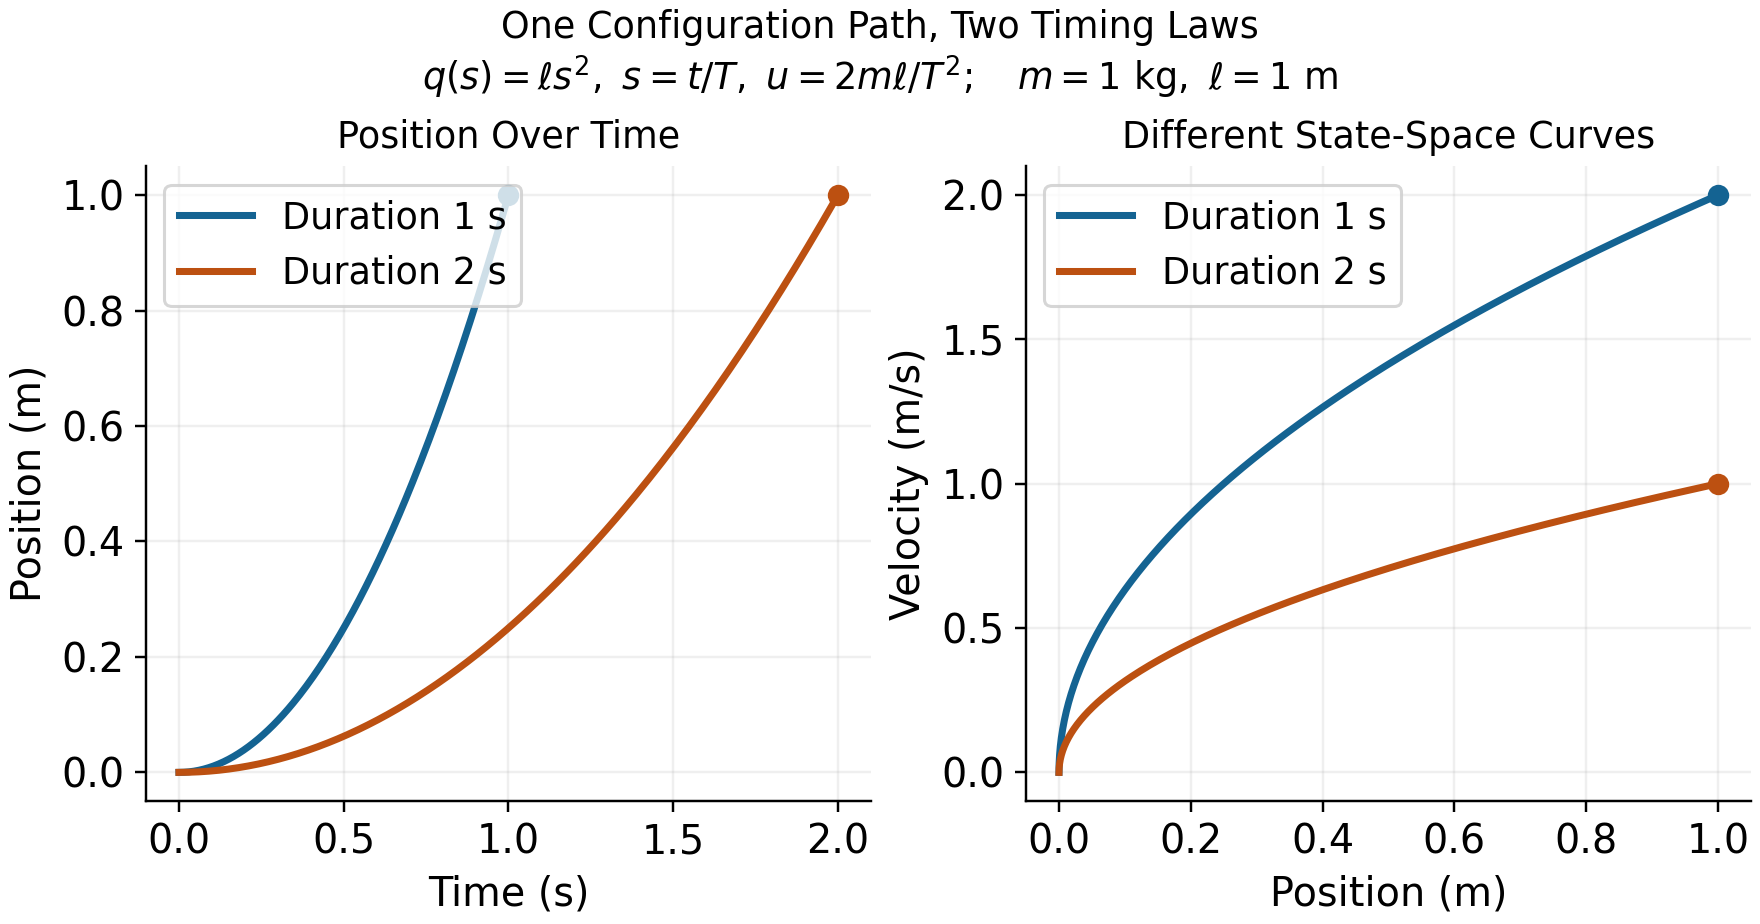
\includegraphics[width=\linewidth]{../The_Geometry_of_Motion/figures/motion_path_timing.png}
\caption{One Configuration Path, Two Timing Laws, and Different State Trajectories. Curves End at the Same Position With Different Velocities.}
\label{fig:motion_path_timing}
\end{figure}

The example uses a prescribed clock-based phase. Estimating phase from the
configuration itself needs care near the stationary start, where $q_d'(0)=0$.
In a swing, a coordinate that reverses at the top of the backswing cannot serve
as a globally increasing phase through that reversal without a different
construction. A useful phase must be defined on the intended interval, be
observable from the chosen state or measurements, and have the required
regularity and progress properties.

\section{Choose a Meaningful Metric and Phase}

A raw norm of position and velocity coordinates mixes different units. Even
among positions, changing metres to centimetres changes an unweighted norm.
One local choice is
\begin{equation}
 \|e\|_W^2=e^TWe,\qquad W=W^T\succ0,
 \label{eq:motion_metric}
\end{equation}
with weights and scales declared according to the desired interpretation.
Under an invertible linear coordinate change $\widetilde e=Se$, the same
quantity uses $\widetilde W=S^{-T}WS^{-1}$. Keeping $W$ unchanged while changing
units generally changes the specification. A physically motivated metric or
scaled output error can be useful, but neither is automatically a clinical
risk measure or an empirical measure of human effort.

On a configuration manifold, subtraction is a local coordinate operation;
rotations, for example, need compatible charts or a chosen local logarithmic
error. The mass matrix defines a kinetic-energy metric on configuration
velocities, not by itself a unique distance on the entire augmented state
including angles, velocities, activation, and other quantities.

For an embedded regular reference curve $\gamma(s)$ in a scaled state chart,
one possible local phase is
\begin{equation}
 s_*(x)\in\arg\min_s\frac12(x-\gamma(s))^TW(x-\gamma(s)).
 \label{eq:motion_projection_phase}
\end{equation}
At an interior minimizer with constant $W$,
\begin{equation}
 \gamma'(s_*)^TW(x-\gamma(s_*))=0.
 \label{eq:motion_phase_orthogonality}
\end{equation}
A sufficiently small tubular neighborhood of a suitably regular embedded curve
can make the projection unique and smooth. That conclusion is local. At the
center of a circle every point on the circle is equally close; self-intersections,
nearby branches, zero tangents, or a finite arc's endpoints can invalidate the
assumed phase chart. A constrained endpoint minimizer need not satisfy the
interior orthogonality equation.

Transverse coordinates need not use nearest-point orthogonality, but must form
valid local coordinates together with phase. If the state dimension is $d$,
there are locally $d-1$ transverse coordinates around a regular one-dimensional
curve. This coordinate count is different from the number of actuators and
from the dimension of a task-equivalent set.

\section{Stability, Attraction, and Finite Motion}

Lyapunov stability means sufficiently small initial errors remain small over
the stated time domain. It does not by itself mean convergence. Asymptotic
stability adds attraction as time tends to infinity. Exponential stability adds
a quantitative decay bound with specified constants. These distinctions apply
to equilibria and have corresponding trajectory and orbital formulations; see
\href{https://underactuated.mit.edu/lyapunov.html}{the MIT Lyapunov analysis notes}.

For a periodic orbit of an autonomous closed-loop system, orbital stability
allows phase displacement while controlling distance to the orbit. A nearby
solution can converge to the orbit without converging to the same clock phase
as a nominal solution. This is useful for periodic motions when phase locking
is not the objective. It is not a general license to change the physical speed
along a prescribed position-velocity curve.

A golf swing studied only up to an impact event is a finite-duration motion.
Its appropriate claims may concern bounded deviation, successful event arrival,
and delivered output tolerances. An infinite-time attraction statement needs
a defined continuation, such as a periodic task or a subsequent stabilization
phase. A finite reference arc is not an invariant orbit once the motion leaves
its endpoint. Bounds on a finite interval should not be renamed asymptotic
stability without that missing structure.

For example, $\dot e=e$ gives $e(t)=e(0)e^t$. On a fixed interval $[0,T]$,
choosing $|e(0)|<\varepsilon e^{-T}$ keeps $|e(t)|<\varepsilon$. This finite-time
bound holds even though errors amplify and the origin is unstable on the
infinite time axis. A useful swing robustness result should therefore report
the permitted initial/measurement uncertainty, the amplification or decay,
the time or event interval, and the terminal output bound.

Orbital analysis still uses Lyapunov functions. For an explicit example,
consider $\dot x_1=x_2$, $\dot x_2=-x_1+u$. The unit circle is a nominal orbit
with $u_d=0$. Put $r^2=x_1^2+x_2^2$ and choose
\begin{equation}
 u=kx_2(1-r^2),\qquad
 V=\tfrac14(r^2-1)^2,\qquad
 \dot V=-k x_2^2(r^2-1)^2\leq0,
 \quad k>0.
 \label{eq:motion_orbit_example}
\end{equation}
On a sufficiently small compact annulus around the unit circle, the largest
invariant subset of $\dot V=0$ is the circle itself. Points with $x_2=0$ away
from the circle do not remain there, since $\dot x_2=-x_1\ne0$; the origin is
excluded by the annulus. Lyapunov and invariance arguments then establish local
orbital attraction and stability. They do not establish phase locking or global
attraction from the origin. The
\href{https://underactuated.mit.edu/limit_cycles.html}{MIT limit-cycle treatment}
and \href{https://arxiv.org/abs/1010.2241}{Manchester's transverse-dynamics analysis}
provide the broader framework.

\section{Verifying a Motion Tube}

A time-varying tube can be defined by
\begin{equation}
 \mathcal T(t)=\{x:V(x,t)\leq\rho(t)\}.
 \label{eq:motion_tube}
\end{equation}
For example, $V$ may measure weighted tracking error. Selecting $\rho(t)$ to
be small near impact expresses a desired tolerance. It does not show that the
closed-loop motion can stay inside the tube. Even $\dot e=0$ leaves a shrinking
tube when initialized on its boundary: constant error cannot fit inside an
arbitrarily decreasing allowed radius.

Suppose the closed-loop dynamics is well posed with admissible inputs,
$V$ and $\rho$ are continuously differentiable, and the tube has a regular
boundary on the domain of interest. For disturbances $d$ in a declared set
$\mathcal D$, a robust inward-boundary condition is
\begin{equation}
 \partial_t V+\nabla_x V^Tf(x,k(x,t),d,t)\leq\dot\rho(t)
 \quad\text{when }V(x,t)=\rho(t),\quad\forall d\in\mathcal D.
 \label{eq:motion_tube_boundary}
\end{equation}
Together with the appropriate regularity and initial membership, this supports
forward invariance over the specified interval. The derivative must include
reference motion and changing metric weights. If $V$ and $\rho$ are indexed
by phase, their derivatives involve the actual $\dot s$; it cannot silently
be replaced by one. Nonsmooth profile corners or hybrid resets need their own
one-sided or transition conditions.

A scalar example makes the effort and disturbance limit explicit. Let
$\dot e=-ke+d$, $|d|\leq\bar d$, and require $|e|\leq r(t)$. On either boundary,
a sufficient condition is
\begin{equation}
 \dot r\geq-kr+\bar d.
 \label{eq:motion_radius_condition}
\end{equation}
For $k=2$, $\bar d=0.1$, and $r(0)=1$ in declared scaled units, the tight
comparison radius is $r(t)=0.05+0.95e^{-2t}$. Constant worst-direction
disturbances attain its two boundaries. The nonzero limiting radius follows
from the disturbance bound and available correction rate. A drawing that
shrinks to zero would not certify this disturbed system.

For an impact specification, also require that every relevant pre-impact
boundary state allowed by the verified tube maps into $\mathcal Y$, and that
the intended event is reached. A phase estimate bounded below by
$\dot s\geq\alpha_{\min}>0$ can supply a progress bound on an appropriate
interval; distance to a path alone cannot. Actuator saturation, sensor delay,
contact feasibility, and uncertainty in the model must be included in the
claimed guarantee. A verified model tube is still a statement about that model
and its declared uncertainty set, not automatic validation on golfers.

\section{Input Rank and Reachability}

For an $n$-coordinate mechanical model with $m<n$ effective inputs, rank limits
instantaneous input acceleration directions. It does not imply that all feasible
states lie on a surface of dimension $2m$. In a state model, drift and input
directions evolve as the system moves; their effect over time can provide
additional reachable directions. The underactuation chapter develops the
associated feasibility and reachability questions.

A concrete counterexample uses two unit masses, one grounded spring, and one
coupling spring, all with unit coefficients. In scaled coordinates,
\begin{equation}
 \ddot q+Kq=bu,\qquad
 K=\begin{pmatrix}2&-1\\-1&1\end{pmatrix},\qquad
 b=\begin{pmatrix}1\\0\end{pmatrix}.
 \label{eq:motion_coupled_springs}
\end{equation}
There is one applied force. With $x=(q_1,q_2,\dot q_1,\dot q_2)^T$,
\begin{equation}
 \dot x=Ax+gu,\qquad
 A=\begin{pmatrix}0&I\\-K&0\end{pmatrix},\qquad
 g=\begin{pmatrix}0\\0\\1\\0\end{pmatrix}.
 \label{eq:motion_spring_state}
\end{equation}
The controllability matrix $[g,Ag,A^2g,A^3g]$ has determinant $-1$ and rank
four. With unconstrained signed inputs, this linear system is controllable in
its full four-dimensional state space. Input limits restrict the size of
reachable sets and time needed; they do not restore the asserted universal
$2m$ dimension bound.

A single trajectory is itself a one-dimensional curve, but the union of
reachable trajectories and the span of a curve's successive derivatives are
different objects. For the same system with $u=0$ and $x(0)=(1,0,0,0)^T$,
the matrix $[Ax,A^2x,A^3x,A^4x]$ at the initial state also has determinant
$-1$. Thus even an unforced example has four independent time derivatives.
At that regular point, smooth arc-length reparameterization preserves their
rank. Actuator count therefore does not cap the number of independent
Frenet-frame directions at $2m$ either.

The useful golf interpretation is more specific. Coupling can transmit and
redistribute the effects of earlier work and present loads. Whether an effective
wrist coordinate is unactuated, weakly actuated, or actively constrained is a
modeling and measurement question. A rapid release does not prove zero wrist
moment, and passive planar dynamics does not guarantee three-dimensional face
squaring. Force, joint moment, mechanical power, and muscle activation must be
kept distinct when testing such hypotheses.

\section{Reliability and Performance}

A path error, a delivery error, and a ball-dispersion measure are different
costs. Choose the one that represents the study, then state how the others
enter the model. Both regulation and trajectory problems can use cost
functionals over an entire history; neither is restricted to a single
instantaneous error value.

For a specified stochastic model and admissible policy $\pi$, one possible
criterion is
\begin{equation}
 \begin{aligned}
 J_\pi&=\phi(y_e)+\int_0^{t_e}\ell(x(t),u(t))\,dt,\\
 \min_\pi\quad&\mathbb E[J_\pi]+\lambda\operatorname{Var}(J_\pi),
 \qquad\lambda\geq0.
 \end{aligned}
 \label{eq:motion_risk_objective}
\end{equation}
The cost and its units, disturbance distribution, event definition, and
constraint handling must be declared. The variance weight has corresponding
units; it expresses a design preference rather than a universal biological
constant. A low variance can accompany a consistently poor mean outcome, so
repeatability alone is not sufficient. Expected cost, tail risk, target-set
probability, and worst-case guarantees answer different questions.
If the intended event is not reached by an allowed horizon, define a failure
cost or constraint; silently discarding those trials changes the question.

A candidate policy may use feedback, a learned reference, or both. Comparing
policies requires recomputing the motion, loads, event time, and output in each
branch. Reusing a measured state or reaction history after the intervention
changes the trajectory can invalidate the comparison. Experimental perturbations
and held-out predictions can test a model; fitting one observed motion does not
establish that the nervous system optimized the proposed criterion.

A practical golf investigation can proceed as follows:
\begin{enumerate}
\item Define the delivered output, its tolerance, and the ball/contact model
      used to connect that output to performance.
\item Declare the mechanical boundary, contact modes, state variables, input
      meaning, parameter uncertainty, and available measurements.
\item Construct compatible nominal states and inputs. Check closure, timing,
      actuator limits, work, and contact feasibility before optimizing a path.
\item Model disturbances and measurement/actuation delays. Compare finite-time
      or event-based output sensitivity and verify any proposed tube condition.
\item Test predictions on independent swings or perturbations, including
      uncertainty in event timing and the inferred loads.
\item Separate demonstrated mechanical identities, validated predictions,
      physiological interpretations, and proposed coaching or design hypotheses.
\end{enumerate}

This is the role of the subsequent chapters: curve geometry describes motion;
configuration manifolds describe compatible coordinates; transverse analysis
and underactuation constrain candidate designs; optimization and robustness
analysis evaluate them; learning and experiments test how well they transfer.
The later golf case study is a modeling proposal unless supported by a complete
specified model, reproducible results, and validation data. The framework's
value comes from making the links testable.

\section{Chapter Exercises}

\begin{enumerate}
\item Specify an impact-event output set that distinguishes clubhead speed,
      face orientation, and impact location. Explain why a terminal target
      does not require stopping there.
\item Derive the error dynamics for the scalar tracking example, then impose
      an input bound and identify where the proposed law becomes infeasible.
\item Reproduce the one-mass timing example. Compare endpoint velocity, input,
      work, and the phase-plane curves for $T=1$ and $T=2$ seconds.
\item For a prescribed pair $(q_d(s),v_d(s))$, derive the compatibility condition
      on $\dot s$ and give an example where arbitrary retiming fails.
\item Rescale a position coordinate from metres to centimetres. Transport the
      error metric and verify that the weighted distance remains unchanged.
\item Show why nearest-point phase is not unique at a circle's center and why
      a finite arc's endpoint needs a separate projection condition.
\item Derive the scalar robust-radius condition and integrate its two
      worst-direction disturbance cases. Explain the nonzero limiting radius.
\item Verify both rank-four matrices in the spring example. Distinguish
      actuator rank, reachable-set dimension, and a trajectory's derivative span.
\item Verify the orbital Lyapunov derivative and the invariant-set argument.
      Explain why this does not prove phase locking or global convergence.
\item Formulate two different reliability objectives for a golf study. State
      what data would distinguish their predictions and what remains unidentifiable.
\end{enumerate}

\end{document}
